\chapter{Implementation}

    \section{Introduction}
    This chapter provides a brief overview of the hardware used, an overview of
    the implementation architecture as well as descriptions of the Broadcaster
    and Observer GAP role implementations. A brief discussion is provided on the
    necessity of route table entry timers and route maintenance in AODV. Finally,
    a discussion of security considerations for the implementation is provided.

    \section{Hardware}
    The hardware used for the implementation of the attendance tracking application
    is Nordic Semiconductor's nRF51 and nRF52 development kit. This kit is used
    for Bluetooth Low Energy, ANT, and 2.4GHz applications.

    The kit provides access to all I/O and interfaces and has four programmable
    LEDs and push buttons. It also has a Segger J-Link interface commonly used
    for debugging.

    \section{Architecture}
        \subsection{Overview}
    The attendance tracking application was implemented using the Nordic SDK \cite{nordic_sdk}.
    The Nordic SDK exposes all the functionality of the BLE stack, such as functions
    to start and stop advertising and scanning, in addition to various device modules
    such as software timers. Custom scanning and advertising files were created
    to encapsulate the available functionality in the SDK, mainly to initialise
    parameters, start, stop, and in the case of advertising, to update the advertisement
    packet currently being broadcast.

    An AODV module was written which sits on top of the Nordic SDK. The AODV module
    contains packet type definitions and functions to send and process control
    packets. These functions adhere to the relevant areas of the AODV specification
    \cite{RFC3561}. A simplified version of the architecture is illustrated in
    \ref{fig:architecture}.

    \FloatBarrier
    \begin{figure}[ht]
      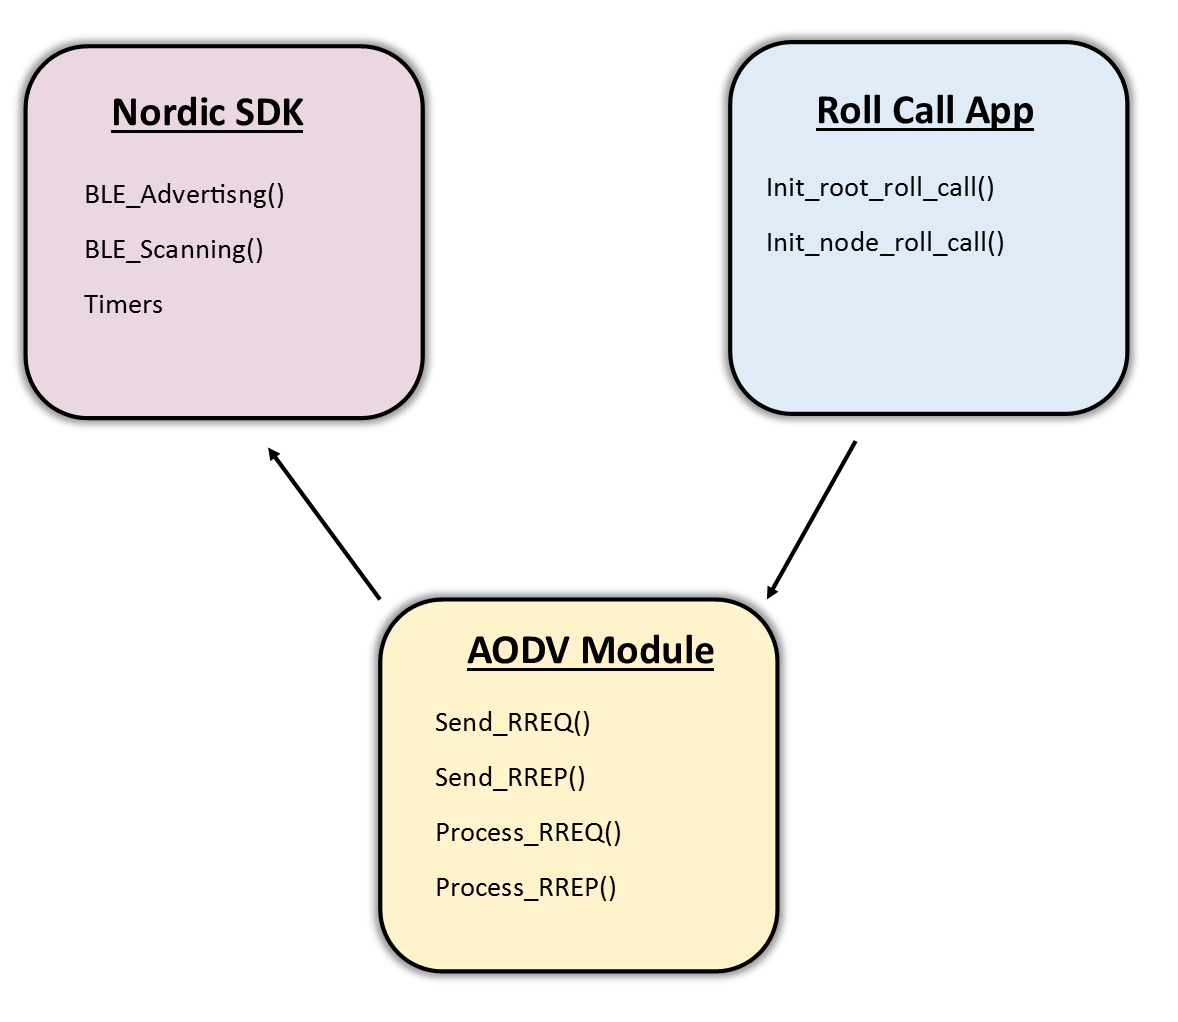
\includegraphics[scale=0.25]{Images/chapter4/architecture.png}
      \caption{Implementaion Architecture}
      \label{fig:architecture}
    \end{figure}
    \FloatBarrier

    The AODV module contains a file which encapsulates packet management and
    functionality. This includes high level structures for RREQ and RREP packets,
    functions to convert these high level structures to and from byte arrays for the
    BLE stack, utility functions to generate packets, copy packets, access individual packet
    bytes, and finally, functions for improved debugging.

    The module contains a file which encapsulates routing table management and
    functionality. This includes a structure for routing table entries, and functions
    for routing table lookups and removals.

    The module contains a main file (aodv\_module.h) which encapsulates the core
    functionality of AODV. This includes module initialisation and reset functions,
    functions to send and process RREQs and RREPs, a function to process advertisement
    reports specific to AODV, timer handlers and a number of global static member
    data such as a list of routing table entries as the routing table, a list of previously
    received packets, and a packet buffer made from a first-in-first-out queue.

      \subsection{Broadcasting}
    Figure \ref{fig:broadcaster} illustrates the flow of execution for the broadcaster
    GAP role implemented in the AODV module.

    \FloatBarrier
    \begin{figure}[ht]
      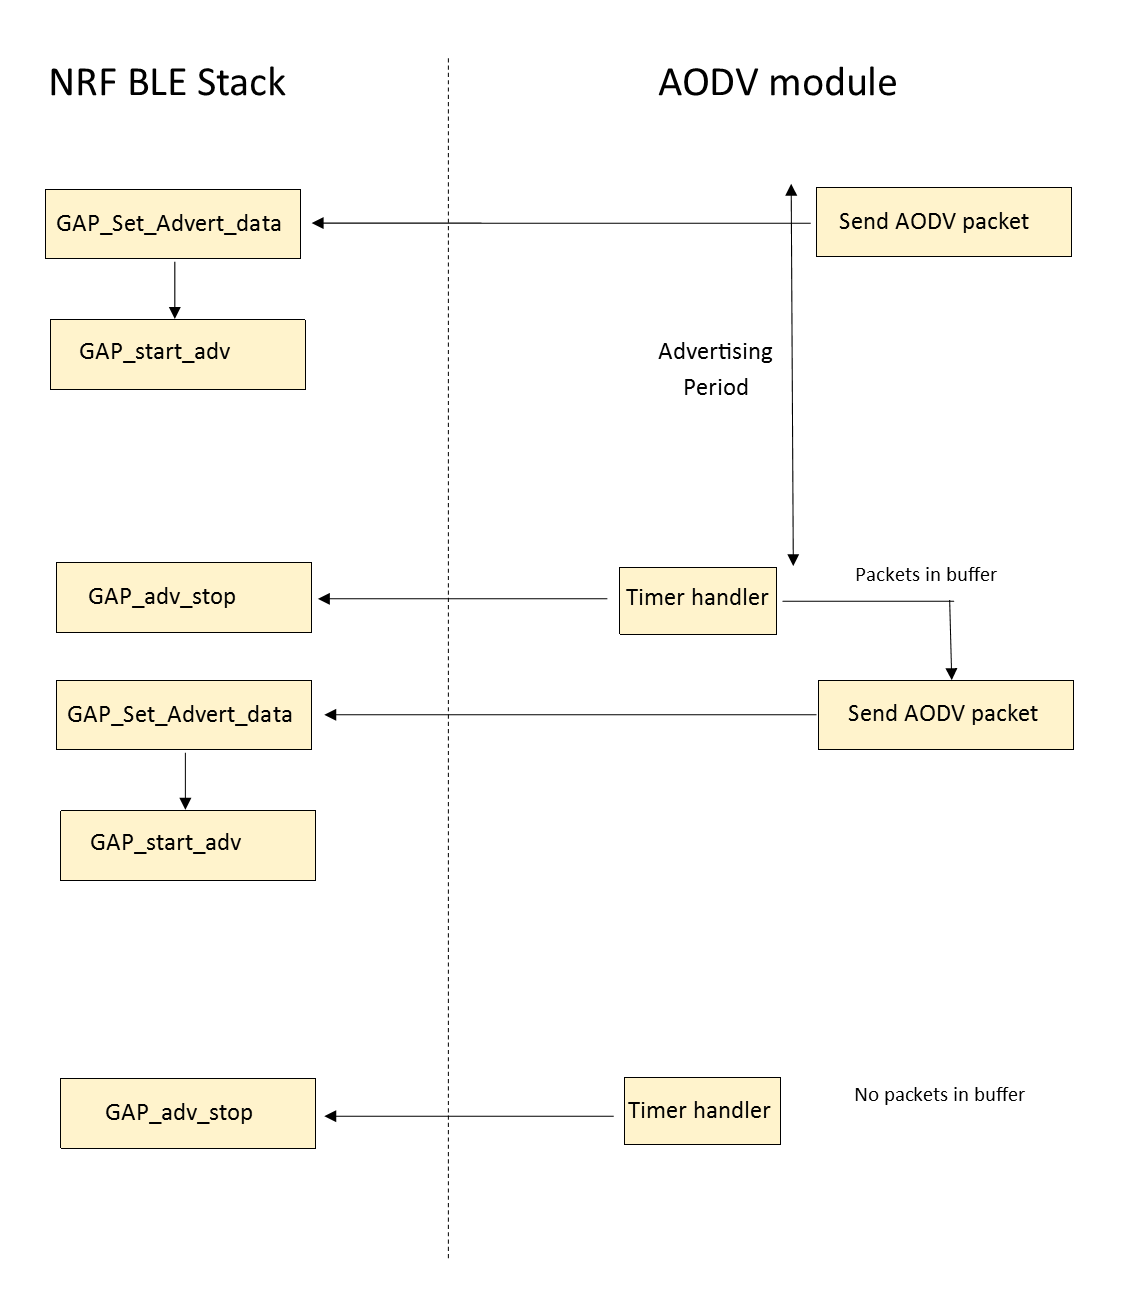
\includegraphics[width=\textwidth]{Images/chapter4/broadcaster_flow.png}
      \caption{Broadcasting Implementation}
      \label{fig:broadcaster}
    \end{figure}
    \FloatBarrier

    As seen in figure \ref{fig:broadcaster}, advertising is initialised and started with the sending of the first RREQ
    packet. Each time a send function is invoked, the packet is placed within
    the packet buffer. When the AODV module is initialised, a recurring timer is
    started which represents the advertising period. Each time the timer
    expires, its handler turns advertisements off, and takes the next packet to
    be sent from the packet buffer. If the buffer is empty, the handler exits,
    leaving advertisements turned off. If there is a packet in the buffer, the
    handler passes it to the appropriate send function (RREQ or RREP).

      \subsection{Observing}
    Figure \ref{fig:observer} illustrates the flow of execution for the observer
    GAP role implemented in the AODV module.

    \FloatBarrier
    \begin{figure}[ht]
      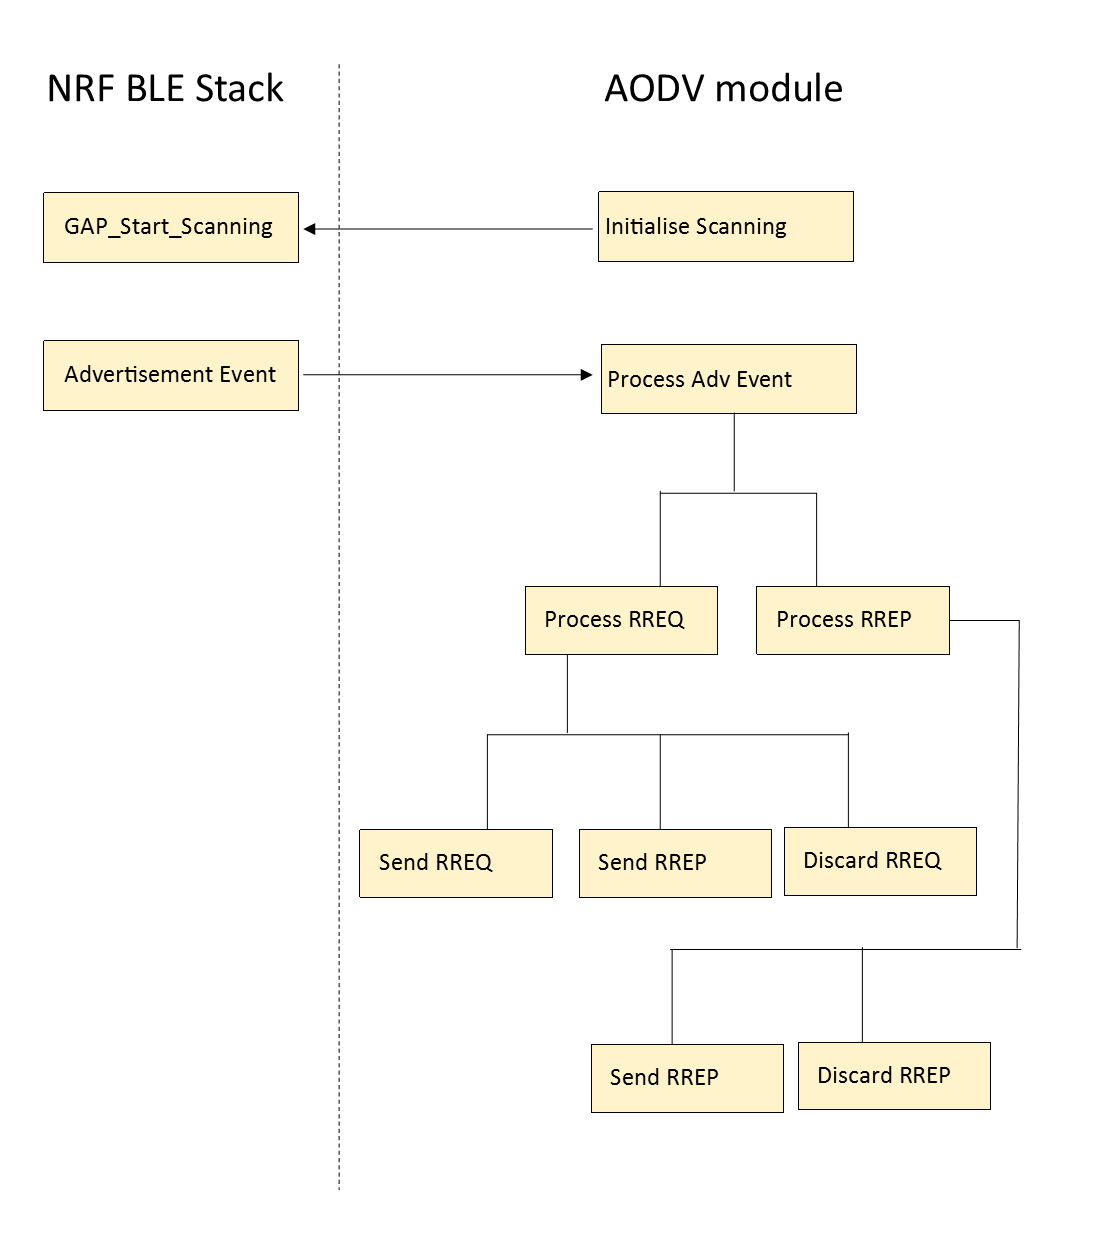
\includegraphics[width=\textwidth]{Images/chapter4/observer_flow.png}
      \caption{Observer Implementation}
      \label{fig:observer}
    \end{figure}
    \FloatBarrier

    As seen in figure \ref{fig:observer}, scanning is initialised and started during
    the initialisation of the AODV module. All devices scan throughout the
    lifetime of the protocol. The BLE stack generates an advertisement event
    when an advertisement packet is scanned. This generated event contains the
    actual packet and all advertisement events are processed by the AODV module.
    the packet is sent to a processing function based on the type of advertisement
    (RREQ/RREP).

    When processing RREQs, to prevent unnecessary processing, if the
    source address is equal to that of the node, the packet is discarded. This is
    required as the node broadcasting the RREQ may scan the same RREQ a number
    of times, possibly more than the number of surrounding nodes re-broadcasting it
    as they repeatedly advertise the duration of the advertisement period.

    If the node processing the RREQ is not the destination, and does not contain
    a route to the destination in their routing table, they buffer the RREQ for
    re-broadcasting.

    If the node processing the RREQ is the destination or has a route to the destination
    in their routing table, they generate a RREP and send it to the source of the RREQ.

     \subsection{Routing table}
    Entries in an AODV routing table have a time-to-live associated with them. This
    is to reduce routing overhead by discarding routes that are not actively being
    used.

    This functionality has not been implemented in the AODV module. The reason for this
    is that the routing table is reset at the start of each period of attendance
    tracking. This is Because nodes are not guaranteed to be in the same location
    with the same neighbours each time the protocol is active, which would result in stale
    routing tables. Another reason is that the implementation was originally targeted
    to be tested in networks with a maximum of 16 nodes so any reduction on routing
    table overhead would be minimal.

    \subsection{Route Maintenance}
    AODV's route maintenance is performed at each node in the network by periodically
    broadcasting HELLO messages. If a node fails to receive a HELLO message from
    another node in one of its routing table entries, the node broadcasts a
    route error message to its neighbours allowing any nodes with an entry to the broken link to
    mark it as invalid.

    Route maintenance is not required when only the route discovery mechanism of
    the protocol is used, and the target networks are semi-static. Not having
    route maintenance still allows for small amounts of mobility, as long as nodes
    stay within range of each other.

    \section{Security Considerations}
    This section discusses some of the security issues with the described implementation
    and possible methods of securing the protocols.

      \subsubsection{Passive Eavesdropping}
    In BLE, when the two devices are initially paired, they derive a long-term key
    using a key-exchange protocol. All communication from that point on is encrypted
    with the derived key. Both AODV based protocols use BLE advertising exclusively,
    no device bonding occurs. Without bonding, it is not possible to achieve secure
    advertising using the BLE stack. It is also worth noting that it is important
    that all nodes in a network can read all packets to update their own routing table
    entries and to properly route packets to the correct destinations. Full packet
    encryption could be used to provide confidentiality and to combat eavesdropping.
    A shared secret key may be programmed into devices which can then be used to
    perform cryptographic operations. This is suitable when application distribution
    is controlled i.e. organisation ID cards with a built in microcontroller.

      \subsubsection{Identity Tracking}
    If a BLE device broadcasts a unique id such as its device address, that address
    can be associated with the device owner/user. This enables the physical tracking
    of the user based on the presence of the BLE device. The purpose of the attendance
    tracking application is to associate devices and users during a gathering
    (lecture/conference/fire evacuation), but malicious nodes eavesdropping during
    these gatherings could then perform identity tracking at any time.

    With BLE, the device address can be manually changed. Changing the device address
    at a specific interval can prevent the association of an address and a user. In
    the context of an attendance tracking application, if a root node attempts to
    identify which devices from a list of device addresses are present, a device
    with a changed address would not be considered. If a device changes its address,
    the root node’s address list needs to be updated.
    Separate unique identifiers should be used in addition to device addresses.
    These identifiers can then be encrypted and the device addresses can be changed
    at regular intervals. This way, only those capable of decryption can associate
    an ID from a device with a user.

      \subsubsection{Impersonation Attacks}
    AODV is susceptible to nodes performing malicious activities while masquerading
    as other nodes.

    AODV specification’s \cite{RFC3561} security considerations section advises the
    following in regards to impersonation attacks:
    \begin{itemize}
      \item Route Response (RREP) packets SHOULD be authenticated to prevent spurious
      routes to a desired destination. This prevents attackers masquerading as a
      desired destination and denying service to the destination or inspecting all
      traffic intended for the destination.
      \item Route Error (RERR) packets SHOULD be authenticated to prevent malicious
      nodes from disrupting valid routes.
      \item Keyed-hash Message Authentication Codes (HMAC) MAY be used to authenticate
      messages given a shared secret key. One issue with hashes in the context of
      BLE advertising is the limited packet size. A BLE advertising packet can
      contain 31 bytes of data. AODV RREP packets require 20 bytes of data, leaving
      room for an 11 Byte MAC.
    \end{itemize}

      \subsubsection{Active Attacks in AODV}
    AODV control packets contain hop counts and sequence numbers which are used
    by nodes to identify the freshness of a route. The mutability of these values
    is a vulnerability, in that nodes can modify these values to maliciously
    advertise better routes.

    By deceptively increasing the sequence number in a packet, a fresher route
    to a particular destination can be advertised. By deceptively decreasing the
    hop count, in-efficient routes will be used, increasing network resource usage.
    Authentication using HMACS, as described above, can be used to prevent
    these attacks.
